\chapter{Application}
\section{Data Explanation}
\label{sec:data}
\begin{comment}
We have now laid down the theory of what we want to do describing all of the choices we may need to make, so now we will put it in action. The data that we will apply it to is a dataset from M.D Anderson Cancer Center. The data is a collection of about 1500 patients at MD Anderson who have breast cancer that has metastasized to the brain, about 100 clinically relevant covariates, along with their survival status and time.
\end{comment}
Now that the theory is in place, we can apply it to some real data. The dataset that I chose to analyze is a dataset from MD Anderson Cancer Center, with permission from Dr. Bugano, Dr. Ibrahim, Dr. Hess and <whoever else needs to be thanked>. The IRB protocol is RCR03-0931. This dataset has historical records of 1514 MD Anderson patients who have had breast cancer that has metastasized to the brain. Metastases are often shortened in speech and in paper to the word �mets�. The dataset consists of 111 covariates, with missingness ranging from 0 to 99\%. Some predictors are metadata, and rare tests, so they will not be considered. Ignoring these, the missingness ranges from 0 to 65\%. Included in these are 90 different covariates, a few different treatments, as well as survival endpoints (which are all observed). The data can be broken down into a few broad categories, as can be seen in table \ref{table:cats}.There are too many covariates to completely explain here, but I�ve listed the ones relevant to our models in table \ref{table:importantvars}

\begin{table}[ !ht]
\centering
\begin{tabular}{|c|c|}
\hline
Type                                                                            & Example                                                                       \\ \hline
Subject data                                                                    & Age range, race, date of birth                                                \\ \hline
Cancer data                                                                     & TNM staging, type, receptor status                                            \\ \hline
\begin{tabular}[c]{@{}c@{}}Pre brain mets\\ data\end{tabular}                   & Treatment types                                                               \\ \hline
\begin{tabular}[c]{@{}c@{}}Post brain mets\\ clinical observations\end{tabular} & Seizures, headache, nasuea                                                    \\ \hline
\begin{tabular}[c]{@{}c@{}}Post brain mets\\ data\end{tabular}                  & \begin{tabular}[c]{@{}c@{}}Treatment type, \\ type of brain mets\end{tabular} \\ \hline
Survival data                                                                   & Survival time after brain mets, censoring indicator                           \\ \hline
\end{tabular}
\caption{Data Categories and Examples}
\label{table:cats}
\end{table}

\begin{table}[ !ht]
\centering
\begin{tabular}{|c|c|c|}
\hline
Name        & \begin{tabular}[c]{@{}c@{}}Percent \\ Missing\end{tabular} & Meaning                                                                                                                                             \\ \hline
hrher2      & 5                                                        & \begin{tabular}[c]{@{}c@{}}Categorical variable: The hormonal receptor and \\ HER2 receptor status of the subject\end{tabular}                      \\ \hline
agebrainmet & 0                                                          & Indicator: Age greater or less than 60 at time of brain mets                                                                                        \\ \hline
timedx      & 1                                                         & \begin{tabular}[c]{@{}c@{}}Indicator: Time (years) from breast cancer diagnosis to brain\\ mets diagnosis greater or less than 6 years\end{tabular} \\ \hline
site5       & 1                                                        & Indicator: First metastasis was to brain                                                                                                            \\ \hline
race2       & 0                                                          & Categorical: White, Black, Hispanic, other                                                                                                          \\ \hline
priorn      & 0                                                          & \begin{tabular}[c]{@{}c@{}}Indicator: Number of prior treatments in metastatic setting \\ before brain mets\end{tabular}                            \\ \hline
braintype   & 4                                                        & Categorical: Single, multiple, Leptomeningeal disease                                                                                               \\ \hline
controlled  & 12                                                        & Indicator: Extracranial progression of brain mets                                                                                                   \\ \hline
capeothno   & 18                                                        & \begin{tabular}[c]{@{}c@{}}Indicator: Capecitabine, other, or no chemotheraputic\\ treatment. Treatment variable 1\end{tabular}                     \\ \hline
lapatrasno  & 18                                                        & \begin{tabular}[c]{@{}c@{}}Indicator: Lapatinib, Trastuzumab, or no HER2 treatment.\\ Treatment variable 2\end{tabular}                             \\ \hline
os          & 0                                                          & Overall survival (months)                                                                                                                           \\ \hline
dead        & 0                                                          & Indicator: death indicator                                                                                                                          \\ \hline
her2        & 10                                                        & Indicator: HER2 receptor status                                                                                                                     \\ \hline
\end{tabular}
\caption{Table of important covariates to be used in the analysis}
\label{table:importantvars}

\end{table}

To get a feel for how the data is missing, in figure \ref{fig:missingplot} we see a plot of the missingness in the data. 
\begin{figure}[h!]
  \centering
    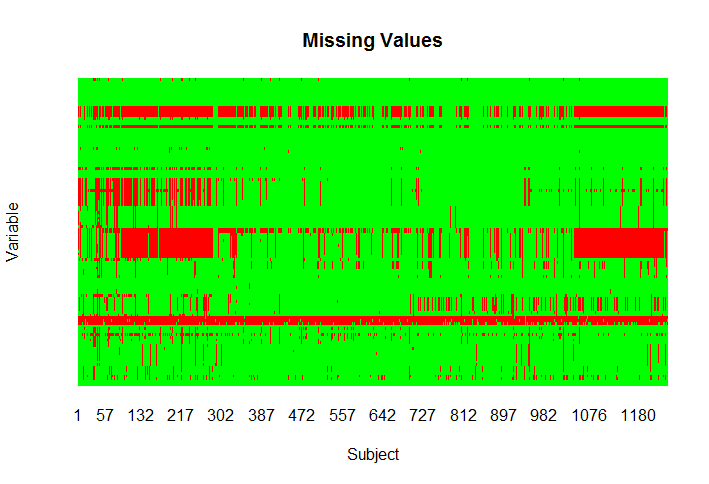
\includegraphics[width=0.8\textwidth]{missingvalues_plot.png}
  \caption{Visualization of missingness in the cancer dataset}
\label{fig:missingplot}
\medskip
\small
Along the horizontal axis is the subject, and the vertical axis is the covariates. \textcolor{green}{Green} denotes observed values whereas \textcolor{red}{red} is missing. The covariates with the highest missingness are three genetic measures, as well as some clinical assessments.
\end{figure}

This data is exemplary for demonstrating thesis ideas because it is a large retrospective study (pulled from a database), survival amenable, has missingness that is a prime candidate for imputation, and has treatment variables that are not given in an RCT.

Our first step is to clearly define what we would like to find. There are many interesting questions we could ask and answer from this data because of the amount of data available, but the question I will focus on here is survival after brain mets from breast cancer in two different settings. In the first, we will explore the treatment effect of Capecitabine (a chemotherapeutic agent) versus other chemotherapeutic agents versus no treatment. In the second, we will look at the effect of two HER2 directed drugs (Lapatinib versus Trastuzumab) versus no HER2 targeted drugs in a subset of the patients who are HER2+.

It isn't vital to understand the entirety of cancer and its treatments for understanding this analysis, but the interested reader may want to look at appendix \ref{app:apdxb} for a very basic overview of breast cancer and the methods of how different drugs work. For a much more detailed analysis and other clinically relevant questions, see the paper by Bugano, Hess, and Berliner. This is the project that this research was forked off of, although it will probably not be published by the time this thesis is. 

\section{Imputation}

We first need to impute the missing data. This is a challenging task, because of the attention and care that needs to be given to imputing about 90 covariates with missing data. But we need these covariates to be imputed properly for many reasons, such as; they have the potential to be useful as predictors for other covariates, they might be something we are actually analyzing (now or later), we have spent the money to collect the data, and it strengthens the MAR assumption. As well, it is my opinion (and probably a consensus among applied statisticians) that is better to have too many covariates than not enough. After all, variable selection can be performed if there are too many covariates. 

Our data is quite high dimensional, and there are a many binary variables as well as a handful of strictly positive covariates, thus JM imputation seems inappropriate. Instead, FCS models seem better suited. We will be using the R package mice \cite{VanBuuren2011} because it is easy to use yet powerful.  There are other software implementations in different languages (such as PROC MI in SAS, ICE in Stata, and package mi in R), but I found mice to be the most flexible while also being powerful and easy to use.

The model is set up by hand, following the advice from \cite{VanBuuren2011}. It took about three weeks to set up and check. This was because the number of covariates was huge, and checking the imputations after a change was time consuming. It would not take this long for a smaller dataset. Creating valid imputations is a skill that lies somewhere between an art and a science, so it takes the theory to know what to do, and trial and error to see if you've done it correctly.

The first task we need to do is to assess the missing data mechanism. As we have discussed before, there is no formal statistical test to determine what the mechanism is. It is very unlikely that the data is MCAR (which we typically associate with random/accidental deletion), so it is between MAR and MNAR. We have so many different covariates, and it could reasonably be assumed that the missing data we have could be explained by the type of disease, its stage, the subject's age, their standardized assessment, and their survival time, among other things which we have collected. So it would be reasonable to assume that the missing data mechanism is MAR, and thus imputation can be confidently used.

For each covariate with missingness, we need to decide the form of the imputation model that will be used for imputation, and what predictors will be used in it. Most of the covariates that needed imputation were either binary or categorical, so the most popular model chosen were logistic regression, multinomial logit regression, or predictive mean matching. The method that was most appropriate for each situation was chosen. The continuous variables were often selected via regression or predictive mean matching. I decided to be very forgiving, and use nearly every reasonable predictor for each missing covariate. I did this to bolster the MAR claim, and avoid variable selection. Van Buuren proposes measures called influx and outflux to determine how worthy and connected each covariate will be as a predictor \cite{VanBuuren2012}. An ideal variable to use as a predictor would be one with an influx near zero and outflux near one. I used all predictors except those that had very poor influx and outflux. Unsurprisingly, the covariates with poor influx and outflux were those who had high missingness or poor relatedness to the rest of the data, as can be seen in table \ref{table:flux}.

\begin{table}[ !ht]
\centering
\begin{tabular}{rrrr}
  \hline
 & Percent Observed & influx & outflux \\ 
  \hline
ki67 & 0.17 & 0.83 & 0.12 \\ 
  brca & 0.05 & 0.95 & 0.04 \\ 
  p53 & 0.01 & 0.99 & 0.01 \\ 
  symptoms & 0.59 & 0.37 & 0.35 \\ 
  seizures & 0.58 & 0.38 & 0.34 \\ 
  headaches & 0.58 & 0.38 & 0.34 \\ 
  nausea & 0.58 & 0.38 & 0.34 \\ 
  chocking & 0.58 & 0.38 & 0.34 \\ 
  balance & 0.58 & 0.38 & 0.34 \\ 
  weakness & 0.58 & 0.38 & 0.34 \\ 
  language & 0.58 & 0.38 & 0.34 \\ 
  cognition & 0.57 & 0.38 & 0.34 \\ 
  ECOG & 0.35 & 0.62 & 0.16 \\ 
  gpaecog & 0.35 & 0.62 & 0.16 \\ 
  gpasum & 0.31 & 0.65 & 0.11 \\ 
   \hline
\end{tabular}
\caption{Percent observed and influx and outflux of the worst predictors. Ki67, brca, and p53 are cancer markers, ECOG and GPA are performance scores}
\label{table:flux}
\end{table}

Once the model and predictor choices were made, the imputations were run and tuned, and checked by trial and error. This took a considerable amount of time, because after every change made, the algorithm needed to be reran and the convergence and imputations needed to be assessed. As well, changes in model specification were rarely localized to that variable, and often affected others. 

For the final MI dataset, it was decided to impute $m=50$ datasets and 40 iterations for each. Mice generally converges quickly (within 5 or 10 iterations), but by setting the number of iterations so high, it is as if we are setting a burn in period, and then taking our sample. The number of imputed datasets was selected to be 50 because in general, the number of datasets should be more than the imputations \cite{Reiter2008}, and while there is no consensus about how many imputations to do, the modern research argues that the more the better. Research by White et. al  says that you should choose $m$ to be about 100 times the percentage of incomplete cases (for the analysis at hand) \cite{White2011a}. The data used in our analysis has about 30\% missingness, so imputing 50 datasets was the chosen number.

After the final model for each covariate with missingness has been set up, we need to run it and save the results. For 50 datasets, 40 iterations, the algorithm runs in about 4 hours, and for 50 datasets with 100 iterations, it took 11.5 hours on a computer with 4 GB of ram and 4 cores. While this seems like a long time, this process only needs to be done once and requires no human interaction, so it can be run overnight and then never need to be touched again. The imputations were run for 100 iterations to see how the run time scaled, as well as to check how the chains behaved and to see how the analyses differed. The results between 50 and 100 iterations were very similar. As well, there is hardly any confidence to be gained going from 50 to 100, and having such large objects in memory can be harder to work with. This is why 50 MI datasets, iterated 40 times each were chosen.

We need to check our final imputations for convergence and reliability. Convergence is assessed by looking at plots of covariate mean and standard deviation by iteration. Diagnosing convergence for binary and categorical variables is a bit tricky, because the mean of a categorical variable is nonsensical, but we can get a good idea of convergence by looking at if the variance remains constant. And for binary variables, knowing how the groups are coded and looking at where the means are can give us an idea of healthy convergence. For example, if we had a variable coded as 1 for underweight and 2 for overweight, and we expected there to be much more overweight imputations than underweight, seeing a mean of 1.8  (indicating 80\% were imputed as overweight) would be reasonable, but 1.2 would not. According to van Buuren ``the different streams should be freely intermingled with each other, without showing any definite trends. Convergence is diagnosed when the variance between different sequences is no larger than the variance with each individual sequence'' \cite{VanBuuren2011}. There are 80 plots to check, so I cannot show all of them in this paper, I only show some interesting ones as a select few can be seen in figure \ref{fig:traceplot1} and \ref{fig:traceplot2}. Looking at these plots, convergence certainly seems to be the case.  Other authors suggest using a more formal statistical tests such as $\hat{R}$, but since most of our interesting variables are categorical, this does not make much sense. 

\begin{figure}[h!]
  \centering
    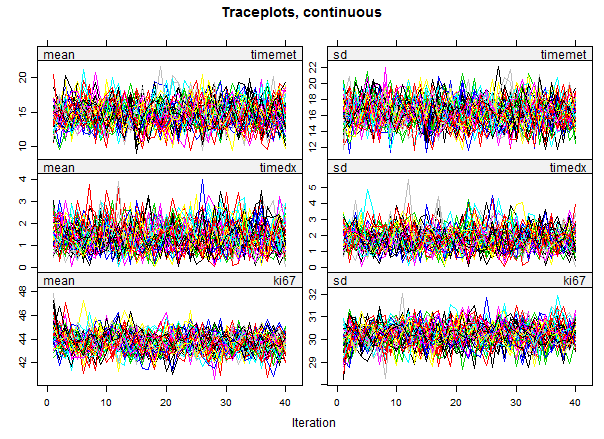
\includegraphics[width=0.8\textwidth]{traceplots1.png}
  \caption{Selected plots of continuous variable imputation mean and standard deviation by iteration}
\label{fig:traceplot1}
\end{figure}


\begin{figure}[h!]
  \centering
    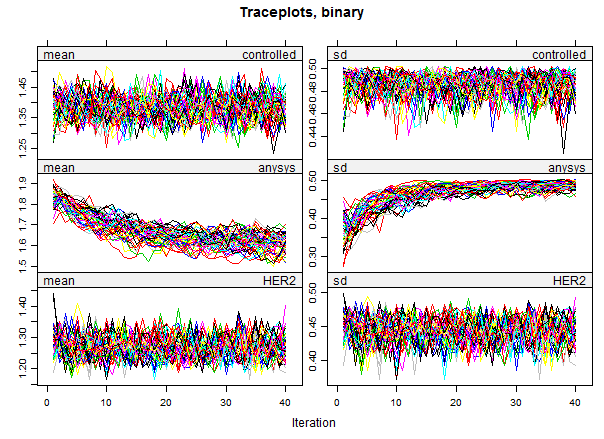
\includegraphics[width=0.8\textwidth]{traceplots2.png}
  \caption{Selected plots of binarys variable imputation mean and standard deviation by iteration}
\label{fig:traceplot2}
\end{figure}

Once the convergence is diagnosed, the validity of the imputations needs to be inspected.  Diagnostic plots are viewed to ensure that the imputed data is similar enough to the real data. Common plots include density plots of each MI dataset compared to the complete cases, as well as bivariate scatterplots for imputed variables. < A few of the plots have been replicated here!!! Still need to do this>. Once again, all of the plots cannot be displayed in this paper, but some important ones are recreated. As we can see, not all of the imputed data follows the distribution of the observed data exactly, but for the majority of the plots, the data look like they could have been real data had they not been missing.

Now that the imputations are done, let�s have a look at the breakdown of the data. In table \ref{table:chartab} we can see how the MI data compares to the available case data, broken down by if the subject had any systemic therapy. As noted before, this was computed via the stacked method because of the percentages.
\begin{table}[!ht]
\centering

\begin{tabular}{|r|l|l|l|l|}
\hline
\multicolumn{1}{|l|}{}                            & \multicolumn{1}{c|}{\begin{tabular}[c]{@{}c@{}}Sys therapy \\ available case\end{tabular}} & \multicolumn{1}{c|}{\begin{tabular}[c]{@{}c@{}}Sys therapy \\ MI\end{tabular}} & \multicolumn{1}{c|}{\begin{tabular}[c]{@{}c@{}}No Sys therapy \\ available case\end{tabular}} & \multicolumn{1}{c|}{\begin{tabular}[c]{@{}c@{}}No Sys therapy \\ MI\end{tabular}} \\ \hline
\multicolumn{1}{|l|}{Age (mean,sd)}               & 51.4(10.8)                                                                                 & 51.2(10.9)                                                                     & 52.7(11.9)                                                                                    & 52.9(11.4)                                                                        \\ \hline
\multicolumn{1}{|l|}{Breast Cancer subtype}       &                                                                                            &                                                                                &                                                                                               &                                                                                   \\ \hline
HR+/HER2-                                         & 27\%                                                                                       & 31\%                                                                           & 28\%                                                                                          & 33\%                                                                              \\ \hline
HR+/HER2+                                         & 19\%                                                                                       & 18\%                                                                           & 12\%                                                                                          & 13\%                                                                              \\ \hline
HR-/HER2+                                         & 22\%                                                                                       & 20\%                                                                           & 15\%                                                                                          & 12\%                                                                              \\ \hline
Triple negative                                   & 32\%                                                                                       & 32\%                                                                           & 45\%                                                                                          & 42\%                                                                              \\ \hline
\multicolumn{1}{|l|}{Prior therapies for stage 4} & 1(0-3)                                                                                     & 2(0-4)                                                                         & 2(0-4)                                                                                        & 2(0-4)                                                                            \\ \hline
\multicolumn{1}{|l|}{Single brain lesion}         & 25\%                                                                                       & 23\%                                                                           & 23\%                                                                                          & 20\%                                                                              \\ \hline
\multicolumn{1}{|l|}{Controlled extra-cranial}    & 40\%                                                                                       & 40\%                                                                           & 35\%                                                                                          & 36\%                                                                              \\ \hline
\multicolumn{1}{|l|}{ECOG 0-1}                    & 84\%                                                                                       & 70\%                                                                           & 53\%                                                                                          & 40\%                                                                              \\ \hline
\multicolumn{1}{|l|}{Local Therapy}               &                                                                                            &                                                                                &                                                                                               &                                                                                   \\ \hline
Resection Alone                                   & 5\%                                                                                        & 5\%                                                                            & 9\%                                                                                           & 7\%                                                                               \\ \hline
SBRT alone                                        & 13\%                                                                                       & 12\%                                                                           & 9\%                                                                                           & 8\%                                                                               \\ \hline
WBRT                                              & 60\%                                                                                       & 59\%                                                                           & 52\%                                                                                          & 53\%                                                                              \\ \hline
Resection/SBRT+WBRT                               & 12\%                                                                                       & 14\%                                                                           & 10\%                                                                                          & 8\%                                                                               \\ \hline
no local therapy                                  & 10\%                                                                                       & 10\%                                                                           & 20\%                                                                                          & 23\%                                                                              \\ \hline
\end{tabular}
\caption{Characteristics of available case data versus MI data}
\label{table:chartab}
\end{table}

\section{Survival Analysis}

Now that the datasets are imputed, we are ready to run our models on them.  Before we begin though, we should check the models on the available cases, to make sure that the model assumptions are met, and to get an idea of how the importance of each part of the model. The available case models (Kaplan-Meier, Cox) were run and the assumptions were checked, and all of them passed. You can see the results, alongside the MI values throughout this section.


It should be noted that in all of our survival analyses, we will be doing a landmark analysis. Landmark analysis means that we don't start the analysis at time 0, rather, we start it at a different time later than 0. In Dr. Hess's words, ``Since the brain mets treatment data was necessarily determined after the diagnosis of the brain met, it is not appropriate to use this data as baseline covariates in the analyses. Only covariates known at the time of diagnosis can be used in this fashion� we can do a landmark analysis by estimating when the vast majority of patients would had their brain met treatment choices started and starting our analyses at this point ''. After speaking with cancer experts (Dr. Bugano and Dr. Ibrahim), this landmark time was determined to be 2 months. 

The first result that we will check is the Kaplan-Meier curves for the imputed data. Noninformative censoring seems to be a valid assumption. The pooled KM estimate was found using Rubin's rules, but under a complimentary log-log transform as suggested by \cite{Marshall2009} to get the survival curves towards normality. The median and confidence interval about it was computed as the median of the upper and lower confidence bands.

The first question we would like to look at is the survival curves for chemotherapeutic drugs. This can be seen in \ref{fig:chemo_km}. The available case and MI analyses look similar, but the MI data seems to give a lower median survival time for the chemotherapeutic drugs. For not taking any chemotherapeutic drugs though, the median increased.

\begin{figure}[h!]
  \centering
    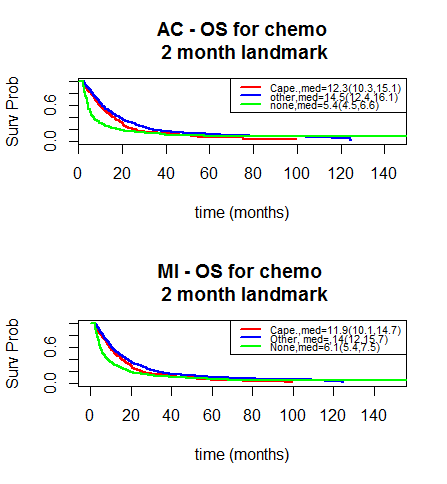
\includegraphics[width=0.8\textwidth]{chemo_km.png}
  \caption{Landmarked Kaplan-Meier curves for chemotherapeutic drugs, AC and MI data}
\label{fig:chemo_km}
\end{figure}


For the HER2 targeted drugs the available case analysis shows that Lapatinib and Trastuzumab are quite close to each other, while having no HER2 directed treatment being much lower. The MI analysis says about the same, but once again gives lower values for the median survival time, as can be seen in figure \ref{fig:her2_km}.

\begin{figure}[h!]
  \centering
    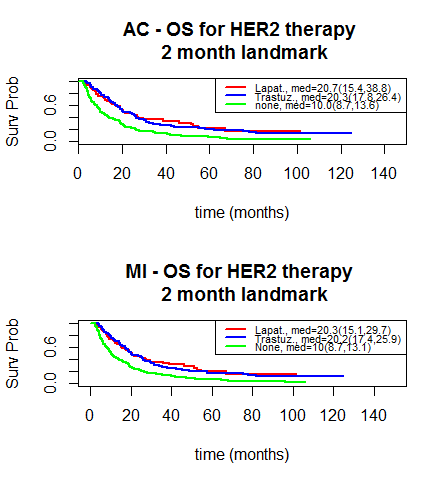
\includegraphics[width=0.8\textwidth]{her2_km.png}
  \caption{Landmarked Kaplan-Meier curves for HER2 drugs, AC and MI data}
\label{fig:her2_km}
\end{figure}


Now that we have a visual of the curves, we would like to see if there is actually a difference between them. To do so, the log rank test needs to be run on them. We can also get an approximation for the log rank test on the MI data via the Wald test on the pooled Cox model fit only on the treatment. Recall that we are not able to get the exact log rank test because in doing so, we would need to compute either the likelihood ratio test or score test, both of which would include calculating the risk set, which is not possible in the MI setting. It has been suggested to pool the chi square statistics via methods presented in Marshall et al 2009, but even they say that this method is poor \cite{Marshall2009}. So, our only real option is to use the Wald test (which is very easy to compute), and use that value as a proxy for the log rank test (they are asymptotically equivalent). <<FIGURE OUT WHICH COMPARISONS I WANT TO USE!!!>>> 

Now that we have estimate of the survival curve, we may set up a model to observe how changes in some baseline covariates change the hazard. We will do this with the Cox Proportional Hazards model. Once we have a baseline model fit and the assumptions met, we can add our treatment variable to see how this affects the hazard.  We first need to fit a reasonable model on the available cases. Speaking with the clinicians, they determined that the covariates listed in table \ref{table:importantvars} were clinically relevant for the baseline model. The available case model will be seen in \ref{}, alongside the MI estimates. 

We need to make sure that the proportional hazards assumption is met in the available case model so we can apply it to the MI data. To check, we visually inspect the Schoenfeld residuals over time. The available cases can be seen in figure \ref{fig:ac_schoenfeld} and the MI can be seen in \ref{fig:mi_schoenfeld}. In the available cases, we have one spline to look at, but for the MI case, all 50 dataset splines are superimposed over eachother. Overall, the assumption of proportional hazards over time seems reasonable, in both the AC and MI analyses. While the splines might not seem exactly straight, it certainly seems reasonable that we could fit a straight edge through the confidence bands.
\begin{figure}[h!]
  \centering
    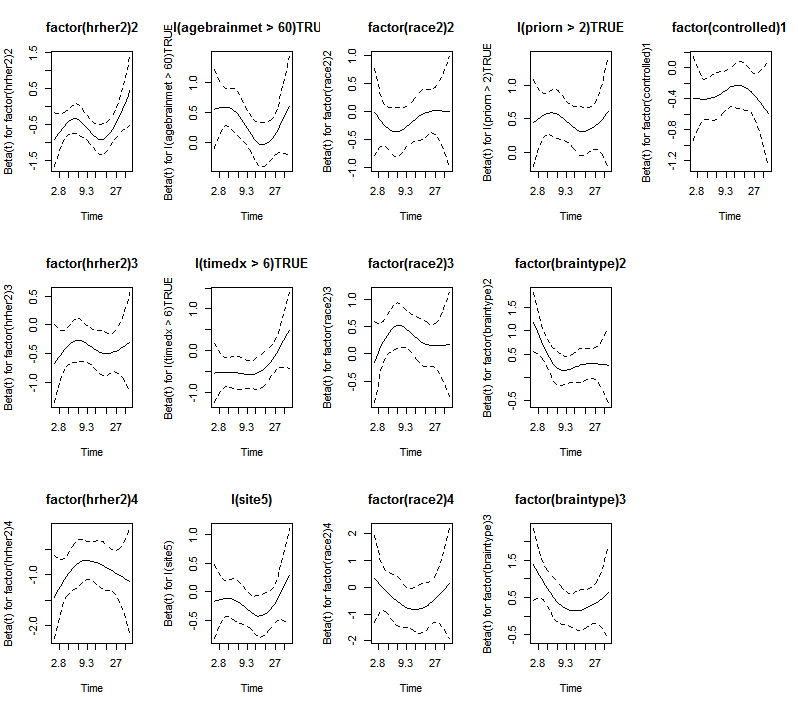
\includegraphics[width=0.8\textwidth]{ac_schoenfeld.png}
  \caption{AC Schoenfeld residuals over time}
\label{fig:ac_schoenfeld}
\end{figure}

\begin{figure}[h!]
  \centering
    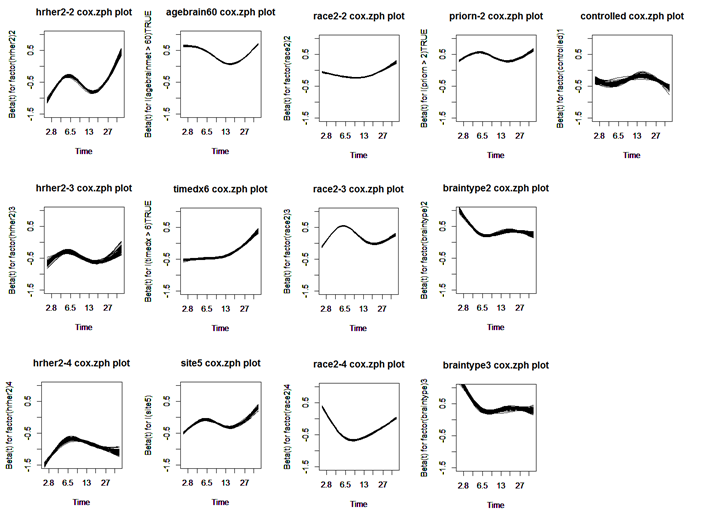
\includegraphics[width=0.8\textwidth]{mi_schoenfeld.png}
  \caption{MI  Schoenfeld residuals over time}
\label{fig:mi_schoenfeld}
\end{figure}


We have verified that the available case analysis seems reasonable, now we can work with the MI data. We fit that same Cox model on all of our imputed data sets, and pool our results via Rubin's rules. We need to verify that we still have proportional hazards though. This is not a straight forward task anymore, since we don't actually have a single model, rather, we have the average of multiple models. We are no longer estimating the parameters by maximizing the partial likelihood; rather we are estimating them based on the average of the coefficients from the MI datasets. There are two ways we can go about verifying the proportional hazards assumption. 

The first is to check the proportional hazards assumptions on the stacked dataset.  To do so, we plot the Schoenfeld residuals over time, and observe the spline fit to it (which should be independent of time). This is a good visual tool, but when running the chi square test to check for the correlation between the coefficient and time, the sample will be artificially too big, and thus we cannot trust the results. 

The correct way to do this is to observe each plot and statistic generated from the 50 datasets to see if the assumptions hold. This may seem like an arduous task when the number of imputed datasets is large, but we can circumvent it by writing <a shiny app to view them>, or <plot all of the splines on one plot>. We can also look at all of the chi square tests for the 50 datasets and 13 variables for each, although there is bound to be some overlap between significance and non-significance due to the multiple testing problem. Overall, our imputed plots are very similar to the plots produced by complete case analysis, to which we have deemed to be acceptable for the proportional hazards assumption. We may now look at the Cox regression coefficients and exponentiate them in order to obtain the hazard ratios, and obtain corresponding 95\% confidence intervals. Looking at <!! table whatever!!> , we can see that some factors  (such as X, Y, Z) force a larger hazard ratio than others. 

We may then add in our treatment variable to see how it affects the hazard, and see how it changes other factors. After doing so, we can see that X does Y. The results can be seen here in a table <of AC vs MI estimates>.

\section{Causal Analysis}

This is the section that needs much more work. I'll only lay the outline here.

Lastly, we will want to draw causal inference, and see what the average treatment effect of each drug is. This is necessary because the data was collected from a database, and we did not have an RCT. As well, this piece of information is what clinicians and laypeople really want�it answers the question of which drug is better. There are many interesting questions that we may ask with this dataset, but here we will only focus on Lapatinib /Trastuzumab /no treatment and Capecitabine/other/none. 

The idea for this part of the analysis is to use propensity score weighting to create a balanced sample, and to be able to treat it as if it was an RCT. Let's do this first on the available cases. To do this though, we need to get an actual propensity score. In talking with the cancer professionals on the project, it was determined that covariates X,Y,Z,� were important  pretreatment variables that needed to be controlled for. In the available case analysis, we see that the standardized bias is <this>. Now, we fit a logistic regression / multinomial logistic model on the treatment status, with the Q variables to get our propensity score. We can look at the <standardized bias> before and after the weighting to ensure that we have controlled properly, and to see if we may go forward. Assuming that we have removed the confounding factors and now have two groups that we can treat like it was an RCT, we may now run our Cox model again, but weight by the IPTW. Once we have done this, we can <observe the results from the AC analysis>.

Now we need to apply this propensity score weighting to the MI data. We discussed before the within and across method, and remarked that we were confined to use the within method, since our treatment variable (lapat/cape) was itself imputed. So the plan will be to fit the Cox models with the inverse propensity score weights discussed in the AC analysis. We need to be sure that the IPTW weighting is still valid in the MI setting though, so we check <standard biased, other things>. Now we may then pool the results via Rubin's rules and analyze is through the Rubin causal model framework. <the results can be seen here>. The results that we can draw from this are X,Y,Z

\begin{comment}
#mdplot
image(is.na(data), main = "Missing Values", xlab = "Subject",
      ylab = "Variable", 
      xaxt = "n", yaxt = "n", bty = "n",col=c("green","red"))
axis(1, seq(0, 1, length.out = nrow(data)), 1:nrow(data), col = "white")
axis(2,tick=FALSE,labels=FALSE)

#traceplots
plot(imp50x40,c("timemet","timedx","ki67"),main="Traceplots, continuous")
plot(imp50x40,c("controlled","anysys","HER2"),main="Traceplots, binary")
#fluxtable
xtable(subset(j,influx>.3&outflux<.5,select=c("pobs","influx","outflux")))

#chemo km
par(mfcol=c(2,1))
#plot it
#available case
plot(survfit(Surv(os,dead)~capeothno,subset=(os>2),data=data),
     mark.time = FALSE,col=c("red","blue","green"),
     main="Available case OS for chemo\n 2 month landmark",
     xlab="time (months)",ylab="Surv Prob",
     xlim=c(0,150),ylim=c(0,1),lwd=2,xaxt='n')
axis(1, at=c(0,20,40,60,80,100,120,140,160))

legend("topright", 
       legend = c("Cape.,med=12.3(10.3,15.1)",
                  "other,med=14.5(12.4,16.1)",
                  "none,med=5.4(4.5,6.6)"),
       col=c("red","blue","green")
       ,lwd=2,cex=.7)

#mi

plot(capeothno_1_mtx[,1],pooled_KM_est1,type="s",col="red",
     main="MI OS for chemo \n 2 month landmark",
     xlab="time (months)",ylab="Surv Prob",
     xlim=c(0,150),ylim=c(0,1),lwd=2,xaxt='n')
axis(1, at=c(0,20,40,60,80,100,120,140,160))
lines(capeothno_1_mtx[,1],pooled_KM_est2, col="blue",type="s",lwd=2)
lines(capeothno_1_mtx[,1],pooled_KM_est3, col="green",type="s",lwd=2)



legend("topright", legend = c(paste0("Cape.,med=",round(median_time1,1),"(",round(lower_time1,1),",",round(upper_time1,1),")"),
                              paste0("Other, med=,",round(median_time2,1),"(",round(lower_time2,1),",",round(upper_time2,1),")"),
                              paste0("None,med=",round(median_time3,1),"(",round(lower_time3,1),",",round(upper_time3,1),")")),
       col=c("red","blue","green"),lwd=2,cex=.7)

#km for her2
par(mfcol=c(2,1))
#plot it

#available case
plot(survfit(Surv(os,dead)~lapatrasno,subset=(os>2&HER2==1),data=data),
     mark.time=FALSE,
     main="AC - OS for HER2 therapy \n 2 month landmark",
     xlab="time (months)",ylab="Surv Prob",
     xlim=c(0,150),ylim=c(0,1),xaxt='n',lwd=2,col=c("red","blue","green"))
axis(1, at=c(0,20,40,60,80,100,120,140,160))


legend("topright", 
       legend = c("Lapat., med=20.7(15.4,38.8)",
                  "Trastuz., med=20.3(17.8,26.4)",
                  "none, med=10.0(8.7,13.6)"),
       col=c("red","blue","green")
       ,lwd=2,cex=.7)


#MI
plot(lapatrasno_1_mtx[,1],pooled_KM_est1,type="s",col="red",
     main="MI - OS for HER2 therapy \n 2 month landmark",
     xlab="time (months)",ylab="Surv Prob",
     xlim=c(0,150),ylim=c(0,1),xaxt='n',lwd=2)
axis(1, at=c(0,20,40,60,80,100,120,140,160))

lines(lapatrasno_1_mtx[,1],pooled_KM_est2, col="blue",type="s",lwd=2)
lines(lapatrasno_1_mtx[,1],pooled_KM_est3, col="green",type="s",lwd=2)



legend("topright", legend = c(paste0("Lapat., med=",round(median_time1,1),"(",round(lower_time1,1),",",round(upper_time1,1),")"),
                              paste0("Trastuz., med=",round(median_time2,1),"(",round(lower_time2,1),",",round(upper_time2,1),")"),
                              paste0("None, med=",round(median_time3,1),"(",round(lower_time3,1),",",round(upper_time3,1),")")),
       col=c("red","blue","green"),lwd=2,cex=.7)

\end{comment}
